\clearpage
\section{Grafici}
\label{sec:grafici}

\subsection{Tempi di risoluzione per \acronimo{cplex}}

\begin{figure}[htb]
	\centering
	\begin{subfigure}[b]{.45\textwidth}
		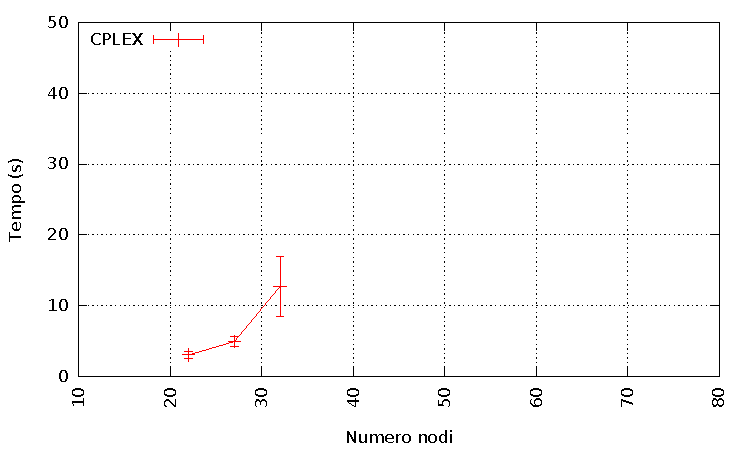
\includegraphics[width=\textwidth]{immagini/cplex_casuali.pdf}
		\caption{Istanze casuali}
		\label{fig:casuali cplex}
	\end{subfigure}
	\quad
	\begin{subfigure}[b]{.45\textwidth}
		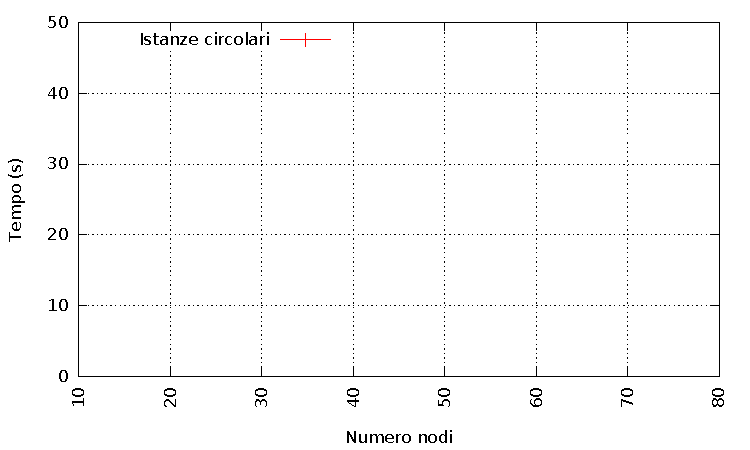
\includegraphics[width=\textwidth]{immagini/cplex_circolari.pdf}
		\caption{Istanze circolari}
		\label{fig:circolari cplex}
	\end{subfigure}
	\caption{Istanza casuali e circolari - \acronimo{cplex}}
	\label{fig:casuali circolari cplex}
\end{figure}

\begin{figure}[htb]
	\centering
	\begin{subfigure}[b]{.45\textwidth}
		\includegraphics[width=\textwidth]{immagini/cplex_cluster_1.pdf}
		\caption{Istanze 1 cluster}
	\end{subfigure}
	\quad
	\begin{subfigure}[b]{.45\textwidth}
		\includegraphics[width=\textwidth]{immagini/cplex_cluster_2.pdf}
		\caption{Istanze 2 cluster}
	\end{subfigure}
	\\
	\begin{subfigure}[b]{.45\textwidth}
		\includegraphics[width=\textwidth]{immagini/cplex_cluster_3.pdf}
		\caption{Istanze 3 cluster}
	\end{subfigure}
	\quad
	\begin{subfigure}[b]{.45\textwidth}
		\includegraphics[width=\textwidth]{immagini/cplex_cluster_4.pdf}
		\caption{Istanze 4 cluster}
	\end{subfigure}
	\caption{Istanze cluster - \acronimo{cplex}}
	\label{fig:cluster cplex}
\end{figure}

\clearpage
\subsection{Tempi di risoluzione per \tabu}

\begin{figure}[htb]
	\centering
	\begin{subfigure}[b]{.45\textwidth}
		\includegraphics[width=\textwidth]{immagini/tabu_4_tempo.pdf}
		\caption{Tenure 4}
	\end{subfigure}
	\quad
	\begin{subfigure}[b]{.45\textwidth}
		\includegraphics[width=\textwidth]{immagini/tabu_5_tempo.pdf}
		\caption{Tenure 5}
	\end{subfigure}
	\\
	\begin{subfigure}[b]{.45\textwidth}
		\includegraphics[width=\textwidth]{immagini/tabu_6_tempo.pdf}
		\caption{Tenure 6}
	\end{subfigure}
	\quad
	\begin{subfigure}[b]{.45\textwidth}
		\includegraphics[width=\textwidth]{immagini/tabu_7_tempo.pdf}
		\caption{Tenure 7}
	\end{subfigure}
	\\
	\begin{subfigure}[b]{.45\textwidth}
		\includegraphics[width=\textwidth]{immagini/tabu_8_tempo.pdf}
		\caption{Tenure 8}
	\end{subfigure}
	\caption{Tempi istanze casuali - \tabu}
	\label{fig:tempi tabu}
\end{figure}

\clearpage
\subsection{Costi delle soluzioni con \tabu}

\begin{figure}[htb]
	\centering
	\begin{subfigure}[b]{.45\textwidth}
		\includegraphics[width=\textwidth]{immagini/tabu_4_costo.pdf}
		\caption{Tenure 4}
	\end{subfigure}
	\quad
	\begin{subfigure}[b]{.45\textwidth}
		\includegraphics[width=\textwidth]{immagini/tabu_5_costo.pdf}
		\caption{Tenure 5}
	\end{subfigure}
	\\
	\begin{subfigure}[b]{.45\textwidth}
		\includegraphics[width=\textwidth]{immagini/tabu_6_costo.pdf}
		\caption{Tenure 6}
	\end{subfigure}
	\quad
	\begin{subfigure}[b]{.45\textwidth}
		\includegraphics[width=\textwidth]{immagini/tabu_7_costo.pdf}
		\caption{Tenure 7}
	\end{subfigure}
	\\
	\begin{subfigure}[b]{.45\textwidth}
		\includegraphics[width=\textwidth]{immagini/tabu_8_costo.pdf}
		\caption{Tenure 8}
	\end{subfigure}
	\caption{Costi istanze casuali - \tabu}
	\label{fig:costi tabu}
\end{figure}

\clearpage
\section{Tabelle}
\label{sec:tabelle}

\subsection{Statistiche istanze casuali risolte con \acronimo{cplex}}

\begin{table}[htb]
	\footnotesize
	\centering
	\caption{Tempi e costi istanze casuali - \acronimo{cplex}}
	\label{tab:casuali}
	\begin{tabular}{cS[table-format=3.4]S[table-format=2.4]S[table-format=2.1]}
	\toprule
	\multirow{2}*{Numero nodi} 	& {Tempo medio} & {Deviazione standard} & \multirow{2}*{Costo medio} \\
								& {(s)}			& {(s)} 				& \\
	\midrule
	11	& 0.2438		& 0.1045	& 55.9 \\
	16	& 0.8337		& 0.3740	& 65.1 \\
	20	& 2.2390		& 1.6470	& 69.6 \\
	25	& 3.6030		& 1.2315	& 76.5 \\
	29	& 6.8557		& 3.9426	& 83.6 \\
	34	& 24.7649		& 13.2507	& 88.9 \\
	38	& 51.4854		& 25.8351	& 91.3 \\
	43	& 101.6627		& 33.2080	& 99.1 \\
	47	& 144.4995		& 24.6324	& 102.2 \\
	52	& 255.3258		& 65.0774	& 107.1 \\
	\bottomrule
	\end{tabular}
\end{table}

\subsection{Statistiche istanze circolari risolte con \acronimo{cplex}}

\begin{table}[htb]
	\footnotesize
	\centering
	\caption{Tempi e costi istanze circolari - \acronimo{cplex}}
	\label{tab:circolari}
	\begin{tabular}{cS[table-format=1.4]S[table-format=3.0]cS[table-format=1.4]S[table-format=3.0]}
	\toprule
	\multirow{2}*{Numero nodi} 	& {Tempo medio} & \multirow{2}*{Costo} 	& \multirow{2}*{Numero nodi} 	& {Tempo medio} & \multirow{2}*{Costo}\\
								& {(s)}			&  						& 								& {(s)}			&  \\
	\midrule
	8	& 0.1228	& 16 & 48	& 1.2384	& 96 \\
	12	& 0.1209	& 24 & 52	& 2.3079	& 104 \\
	16	& 0.0663	& 32 & 56	& 4.1274	& 112 \\
	20	& 0.2185	& 40 & 60	& 4.6480	& 120 \\
	24	& 0.3220	& 48 & 64	& 3.7191	& 128 \\
	28	& 0.2246	& 56 & 68	& 3.6495	& 136 \\
	32	& 0.4750	& 64 & 72	& 3.7701	& 144 \\
	36	& 0.8386	& 72 & 76	& 3.4811	& 152 \\
	40	& 1.8196	& 80 & 80	& 4.2138	& 160 \\
	44	& 1.2220	& 88 & 84	& 6.5727	& 168 \\
	\bottomrule
	\end{tabular}
\end{table}

\clearpage
\subsection{Statistiche istanze cluster risolte con \acronimo{cplex}}

\begin{table}[htb]
	\scriptsize
	\centering
	\caption{Tempi e costi istanze cluster - \acronimo{cplex}}
	\label{tab:cluster}
	\begin{tabular}{ccS[table-format=3.4]S[table-format=2.4]S[table-format=2.1]}
	\toprule
		& \multirow{2}*{Numero nodi} 	& {Tempo medio} & {Deviazione standard} & \multirow{2}*{Costo medio} \\
		&								& {(s)}			& {(s)} 				& \\
	\midrule
	\multirow{10}*{\begin{sideways}1 cluster\end{sideways}} & 2	& 0.0009	& 0.0001	& 8.7 \\
	& 4	& 0.0514	& 0.0195	& 16.0 \\
	& 5	& 0.0734	& 0.0310	& 18.9 \\
	& 7	& 0.1518	& 0.0950	& 22.3 \\
	& 8	& 0.1655	& 0.1044	& 23.1 \\
	& 10	& 0.2061	& 0.1031	& 24.3 \\
	& 11	& 0.2239	& 0.0738	& 25.7 \\
	& 13	& 0.4562	& 0.2643	& 26.8 \\
	& 14	& 0.5176	& 0.1663	& 28.6 \\
	& 16	& 0.7303	& 0.4115	& 30.4 \\
	\midrule
	\multirow{10}*{\begin{sideways}2 cluster\end{sideways}} & 4	& 0.0723	& 0.0370	& 38.1 \\
	& 8	& 0.1715	& 0.0462	& 47.9 \\
	& 10	& 0.3779	& 0.1874	& 50.9 \\
	& 14	& 1.3264	& 0.6812	& 55.5 \\
	& 16	& 1.6585	& 1.0877	& 57.6 \\
	& 20	& 3.9322	& 2.1850	& 60.5 \\
	& 22	& 4.2853	& 2.8440	& 63.1 \\
	& 26	& 7.7065	& 3.8624	& 64.7 \\
	& 28	& 14.4487	& 10.7130	& 66.1 \\
	& 32	& 52.5417	& 73.9963	& 70.7 \\
	\midrule
	\multirow{10}*{\begin{sideways}3 cluster\end{sideways}} & 6	& 0.0969	& 0.0385	& 44.2 \\
	& 12	& 0.5026	& 0.2955	& 54.9 \\
	& 15	& 1.0327	& 0.6484	& 58.1 \\
	& 21	& 2.8062	& 1.7474	& 65.2 \\
	& 24	& 3.3463	& 1.3332	& 68.0 \\
	& 30	& 12.4023	& 8.0275	& 74.9 \\
	& 33	& 23.2862	& 15.1886	& 77.7 \\
	& 39	& 51.0216	& 21.6250	& 83.3 \\
	& 42	& 92.3221	& 17.6381	& 85.8 \\
	& 48	& 137.4311	& 44.2163	& 89.3 \\
	\midrule
	\multirow{10}*{\begin{sideways}4 cluster\end{sideways}} & 8	& 0.1588	& 0.1086	& 50.7 \\
	& 16	& 0.8943	& 0.4948	& 67.2 \\
	& 20	& 3.1633	& 1.9649	& 72.4 \\
	& 28	& 6.8458	& 4.1326	& 81.0 \\
	& 32	& 16.6601	& 12.6953	& 86.3 \\
	& 40	& 69.2420	& 23.0443	& 96.4 \\
	& 44	& 107.8618	& 25.5995	& 99.9 \\
	& 52	& 227.9986	& 53.9585	& 107.2 \\
	& 56	& 280.3272	& 61.0582	& 110.7 \\
	& 64	& 625.6605	& 266.3992	& 116.7 \\
	\bottomrule
	\end{tabular}
\end{table}

\clearpage
\subsection{Statistiche istanze casuali risolte con \tabu}

\begin{table}[htb]
	\tiny
	\centering
	\caption{Tempi e costi istanze casuali - \tabu}
	\label{tab:tabu}
	\begin{tabular}{ccS[table-format=1.4]S[table-format=1.4]S[table-format=3.3]S[table-format=1.4]}
	\toprule
		& \multirow{2}*{Numero nodi} 	& {Tempo medio} & {Deviazione standard} & \multirow{2}*{Costo medio} 	& {Deviazione standard}\\
		&								& {(s)}			& {(s)} 				& 								& \\
	\midrule
	\multirow{10}*{\begin{sideways}tabu tenure 4\end{sideways}} & 11	& 0.0040	& 0.0007	& 55.9		& 5.4858 \\
		& 16	& 0.0110	& 0.0021	& 65.855	& 5.7060 \\
		& 20	& 0.0208	& 0.0027	& 70.7		& 4.3839 \\
		& 25	& 0.0335	& 0.0043	& 78.465	& 6.0996 \\
		& 29	& 0.0651	& 0.0153	& 86.41		& 5.4463 \\
		& 34	& 0.1149	& 0.0130	& 91.18		& 6.1521 \\
		& 38	& 0.1541	& 0.0046	& 94.745	& 3.1352 \\
		& 43	& 0.1902	& 0.0058	& 103.485	& 4.9944 \\
		& 47	& 0.2242	& 0.0059	& 107.55	& 3.8716 \\	
		& 52	& 0.2791	& 0.0065	& 113.275	& 4.1192 \\
	\midrule
	\multirow{10}*{\begin{sideways}tabu tenure 5\end{sideways}} & 11	& 0.0044	& 0.00089	& 55.9		& 5.4858 \\
		& 16	& 0.0120	& 0.00151	& 65.42		& 5.4641 \\
		& 20	& 0.0185	& 0.00217	& 70.335	& 4.2735 \\
		& 25	& 0.0331	& 0.00315	& 78.065	& 5.4499 \\
		& 29	& 0.0599	& 0.01498	& 86.005	& 4.0309 \\
		& 34	& 0.1197	& 0.00567	& 91.43		& 5.7485 \\
		& 38	& 0.1491	& 0.00678	& 94.455	& 2.8618 \\
		& 43	& 0.1886	& 0.00527	& 103.07	& 5.1433 \\
		& 47	& 0.2281	& 0.00376	& 106.54	& 4.3268 \\
		& 52	& 0.2828	& 0.01059	& 112.665	& 3.7144 \\	
	\midrule
	\multirow{10}*{\begin{sideways}tabu tenure 6\end{sideways}} & 11	& 0.0047	& 0.0010	& 55.9		& 5.4858 \\ 
		& 16	& 0.0114	& 0.0015	& 65.2		& 5.2475 \\
		& 20	& 0.0211	& 0.0034	& 70.325	& 4.1817 \\
		& 25	& 0.0341	& 0.0047	& 76.76		& 4.9318 \\
		& 29	& 0.0523	& 0.0100	& 86.13		& 5.1482 \\
		& 34	& 0.1183	& 0.0127	& 91.04		& 4.7051 \\
		& 38	& 0.1567	& 0.0052	& 94.235	& 3.8094 \\
		& 43	& 0.1971	& 0.0036	& 102.35	& 4.8162 \\
		& 47	& 0.2332	& 0.0068	& 106.45	& 4.1793 \\
		& 52	& 0.2878	& 0.0077	& 111.505	& 3.9733 \\
	\midrule
	\multirow{10}*{\begin{sideways}tabu tenure 7\end{sideways}} & 11	& 0.0047	& 0.0011	& 55.9		& 5.4858 \\
		& 16	& 0.0118	& 0.0015	& 65.63		& 5.6266 \\
		& 20	& 0.0210	& 0.0017	& 69.745	& 3.9841 \\
		& 25	& 0.0315	& 0.0032	& 77.9		& 5.2005 \\
		& 29	& 0.0641	& 0.0174	& 84.46		& 4.8488 \\
		& 34	& 0.1217	& 0.0084	& 91.075	& 5.8853 \\
		& 38	& 0.1535	& 0.0078	& 93.705	& 3.1860 \\
		& 43	& 0.1933	& 0.0058	& 101.77	& 4.6907 \\
		& 47	& 0.2311	& 0.0057	& 105.8		& 4.1282 \\
		& 52	& 0.2846	& 0.0094	& 111.14	& 3.5792 \\
	\midrule
	\multirow{10}*{\begin{sideways}tabu tenure 8\end{sideways}} & 11	& 0.0047	& 0.0007	& 55.9		& 5.4858 \\
		& 16	& 0.0120	& 0.0016	& 65.5		& 5.5772 \\
		& 20	& 0.0223	& 0.0024	& 70.04		& 4.1890 \\
		& 25	& 0.0347	& 0.0047	& 77.115	& 4.8038 \\
		& 29	& 0.0564	& 0.0113	& 85.115	& 5.0305 \\
		& 34	& 0.1251	& 0.0055	& 90.835	& 5.4048 \\
		& 38	& 0.1526	& 0.0051	& 94.155	& 4.1911 \\
		& 43	& 0.1962	& 0.0056	& 101.995	& 4.5129 \\
		& 47	& 0.2324	& 0.0053	& 105.55	& 3.5185 \\	
		& 52	& 0.2929	& 0.0080	& 110.93	& 3.7861 \\
	\bottomrule
	\end{tabular}
\end{table}

